\section{Directional Change Intrinsic Time Framework}

In this section, we dive into the technical details of the Directional Change (DC) Intrinsic Time Framework. To elaborate on the naming, `Directional Change' describes the \textit{Directional Change Events} identified from a given time series by an algorithm and `Intrinsic Time' is one of the key characteristics of the DC events. We start by addressing such an algorithm in Section \ref{subsec: dc algo}, and we discuss the framework and its intrinsic time ideology in Section \ref{subsec: dc discussion}.

\subsection{The Algorithm for Directional Change Events}\label{subsec: dc algo}
The algorithm in the DC framework operates much like a state machine. Given a univariate time series, it classifies every entry in the time series into \textit{states}. The algorithm's output is thus the same time series but with a state assigned to each entry by the algorithm. The primary goal of such an algorithm is to provide information on directional change events. Moreover, the assignment of states is also the source of many other interesting analyses and implementations carried out under the DC framework. Let an arbitrary time series be $\mathcal{Y}_{t_k} = \{y_{t_i} \}_{i = 1, 2, \ldots, k}$. Then the algorithm $\mathcal{A}^{(DC)}$ can be noted as
\begin{equation*}
    \mathcal{Y}_{t_k}^{(DC)} = \mathcal{A}^{(DC)} (\mathcal{Y}_{t_k} ; \delta, \mathcal{R} (x; y)) = \{ (y_{t_i}, s)\}_{i = 1, 2, \ldots, k}, \; s \in S
\end{equation*}
where
\begin{itemize}
    \setlength\itemsep{-5pt}
    \item $\delta = (\delta_{down}, \delta_{up})$ is a pair of threshold values parameterising the classification
    \item $\mathcal{R} (x; y)$ is a measure of change of value $x$ with respect to a given reference $y$\footnote{For instance, the net return is $\mathcal{R} (x; y) = \frac{x - y}{y}$.}.
    \item $S$ is a set of possible states identified by the algorithm. 
    \item An entry $(y_{t_i}, s) \in \mathcal{Y}_{t_k}^{(DC)}$ signifies the value $y_{t_i}$ being classified as state $s$ by $\mathcal{A}^{(DC)}$.
\end{itemize}
Having consecutive values assigned to the same state means these values form an event with duration. Such events can be \textit{Bullish Trend}, \textit{Bullish Overshoot}, \textit{Bearish Trend}, or \textit{Bearish Overshoot}. By construction of the algorithm, bullish and bearish trends appear alternatively with the gap being filled by an overshoot following the direction of the former trend. An overshoot is essentially the residual of a trend before reaching the start of the next opposite-direction trend. For example:
\begin{align*}
    &\text{bullish trend} \rightarrow \text{bullish overshoot} \rightarrow \text{bearish trend} \rightarrow \text{bearish overshoot} \\
    & \rightarrow \text{bullish trend} \rightarrow \text{bullish overshoot} \rightarrow \text{bearish trend} \cdots.
\end{align*}
In order to mark the events, set $S$ consists of seven possible states that could be assigned to the values in $\mathcal{Y}_{t_k}$:
\begin{enumerate}
    \item[1.] Local Extreme: The starting point of a time series is identified as a local extreme. Other than the starting point, the rest of the local extreme points are the start of a trend and also the end of the previous overshoot. One thing to highlight is that, except for the starting point, all local extrema are only recognisable once its latter trend is identified. In other words, they are determined in hindsight.
    \item[2.,3.] Bullish or Bearish Trend: The value is identified as experiencing a bullish or bearish trend.
    \item[4.,5.] Bullish or Bearish Overshoot: Upon identifying a bullish or bearish trend, the price is at a bullish or bearish overshoot before it reaches a local extreme (or, say, the next trend with the opposite direction).
    \item[6.,7.] Bullish or Bearish DC Confirmation: This value confirms the occurrence and ends a bullish or bearish trend. Note that the end of a bullish or bearish trend is also the end of a DC event and the start of the next one. This is identified by the value that has risen or decreased more than $\delta_{up}$ or $\delta_{down}$ compared to the previously spotted local extreme.
\end{enumerate}
Figure \ref{fig: dc} is a figure we found in Petrov et al. (\citeyear{petrov2018agent}) that illustrates the Directional Change Framework.
\begin{figure}[H]
    \centering
    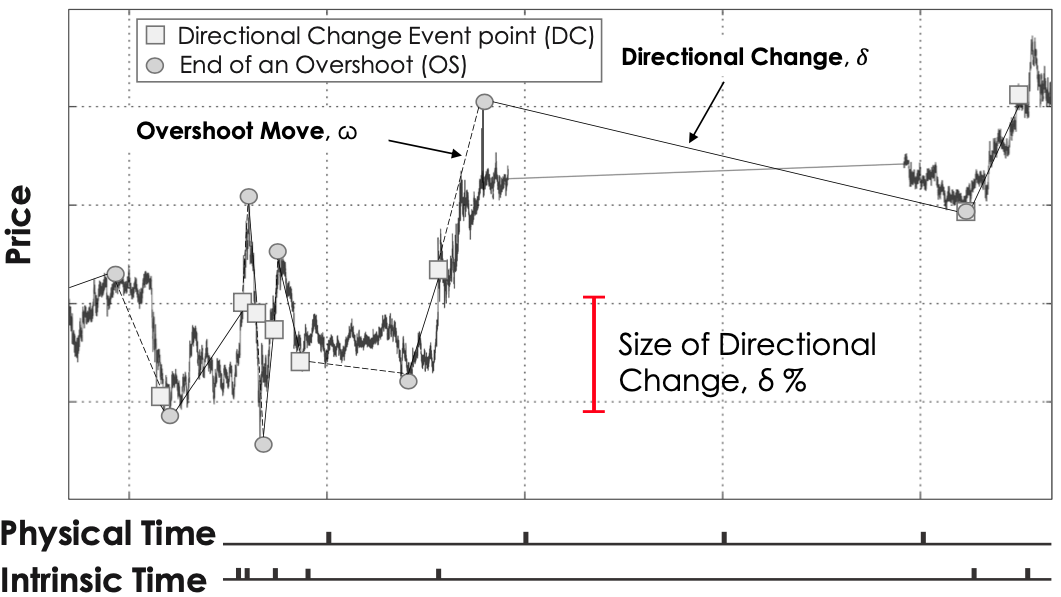
\includegraphics[width=\columnwidth]{dc}
    \caption{Illustration of DC Framework}
    {\raggedright \footnotesize This figure is a direct reference to the one in Petrov et al. (\citeyear{petrov2018agent}). This is an example of an exchange rate price time series and the directional change events identified using an arbitrary symmetric $\delta$ threshold. \par}
    \label{fig: dc}
\end{figure}
See Algorithm \ref{alg: dc} for the detailed pseudocode of $\mathcal{A}^{(DC)} (\mathcal{Y}; \delta, \mathcal{R})$.
\begin{algorithm}
    \caption{The Algorithm for Directional Change Events}\label{alg: dc}
    \begin{algorithmic}
    \State{Input: a time series $\mathcal{Y}_{t_k} = \{y_{t_i} \}_{i = 1, 2, \ldots, k}$}
    \State{Input: a pair of downward and upward thresholds $\delta = (\delta_{down}, \delta_{up})$}
    \State{Input: a return measure $\mathcal{R} (x ; y)$ for a spot value $x$ with respect to a given reference value $y$}
    \State{Initialise current mode to $none$}
    \State{Initialise local extreme $e$ to $none$}
    \For{$y_{t_i} \in \{y_{t_1}, y_{t_2}, \cdots, y_{t_k} \} $}
        \If{$i$ is $1$}
            \State{Update local extreme $e$ to $y_{t_i}$ and move on to the next iteration.}
        \EndIf
        \If{Current mode is $none$}
            \State{$r \leftarrow \mathcal{R}(y_{t_i}; e)$}
            \If{$r \geq \delta_{up}$}
                \State{Mark a bullish trend from the last local extreme to current $y_{t_i}$.}
                \State{Update current mode to $bullish$ and move on to the next iteration.}
            \ElsIf{$ r < \delta_{down}$}
                \State{Mark a bearish trend from the last local extreme to current $y_{t_i}$.}
                \State{Update current mode to $bearish$ and move on to the next iteration.}
            \EndIf
            \State{Mark $y_{t_i}$ to unidentified state.}
        \EndIf
        \If{Current mode is $bullish$}
            \If{$y_{t_i} \geq e$}
                \State{Update the local extreme $e$ to $y_{t_i}$.}
            \EndIf
            \State{$r \leftarrow \mathcal{R} (y_{t_i}; e)$}
            \If{$r \leq \delta_{down}$}
                \State{Update current mode to $bearish$.}
                \State{Mark a bearish trend from the local extreme to the current $y_{t_i}$.}
                \State{Move on to the next iteration.}
            \EndIf
            \State{Mark $y_{t_i}$ as going through a bullish overshoot.}
        \ElsIf{Current mode is $bearish$}
            \If{$y_{t_i} \leq e$}
                \State{Update the local extreme $e$ to $y_{t_i}$.}
            \EndIf
            \State{$r \leftarrow \mathcal{R}(y_{t_i}; e)$}
            \If{$r \geq \delta_{up}$}
                \State{Update current mode to $bullish$.}
                \State{Mark a bullish trend from the local extreme to the current $y_{t_i}$.}
                \State{Move on to the next iteration.}
            \EndIf
            \State{Mark $y_{t_i}$ as going through a bearish overshoot.}
        \EndIf
    \EndFor
    \end{algorithmic}
\end{algorithm}

\subsection{Discussions}\label{subsec: dc discussion}
A directional change event is a downturn or upturn event which is a combination of an overshoot and its consecutive trend\footnote{An overshoot and its consecutive trend have opposite directions.}, and the identification of DC events is the primary goal of the $\mathcal{A}^{(DC)}$ algorithm. Here are some remarks concerning the algorithm and its output.
\begin{enumerate}
    \item Observe that a DC event is considered complete only when the time series has moved passed the threshold set by $\delta = (\delta_{down}, \delta_{up})$ according to measure $\mathcal{R}$. Therefore, higher $\delta$ values lead to fewer total DC events identified by the algorithm and vice versa.
    \item Due to how $\mathcal{A}^{(DC)}$ is parameterised by $\delta$, the number of DC events is negatively correlated to the volatility of $\mathcal{Y}_{t_k}$.
    \item In the event where $\delta_{down} \neq \delta_{up}$, the algorithm is set to have different sensitivity to bullish and bearish trends.
    \item $\mathcal{A}^{(DC)}$ is a deterministic mapping if $\mathcal{Y}_{t_k}$, $\delta$ and $\mathcal{R}$ are given.
    \item As mentioned previously, except for the first one, identifying a local extreme can only be made until its following trend is confirmed. In time series analysis, we say that the process of identifying local extrema uses \textit{look-ahead information}. This means that knowing the past values is not enough; classifying a local extreme does not happen in real-time as the algorithm loops through the values in $\mathcal{Y}_{t_k}$ chronologically.
    \item Let $\mathcal{Y}^{(IT)}_{t_k}$ be the subset of $\mathcal{Y}^{(DC)}_{t_k}$ such that
    \begin{equation*}
        \mathcal{Y}^{(IT)}_{t_k} = \{ (y_{t_i}, s) | s = \text{DC Confirmation} \}_{i = 1, 2, \ldots, k}.
    \end{equation*}
    Then the timestamp set of $\mathcal{Y}^{(IT)}_{t_k}$, which we denote as $t^{(IT)}$, marks the time points where directional change events are confirmed. $t^{(IT)}$ is called the \textit{Directional Change Event-based Intrinsic Time} of $\mathcal{Y}_{t_k}$ based on $\delta$ and $\mathcal{R}$.
\end{enumerate}
